\documentclass[a4paper]{article}
\usepackage[utf8]{inputenc}
\usepackage[spanish, es-tabla, es-noshorthands]{babel}
\usepackage[table,xcdraw]{xcolor}
\usepackage[a4paper, footnotesep = 1cm, width=20cm, top=2.5cm, height=25cm, textwidth=18cm, textheight=25cm]{geometry}
%\geometry{showframe}

\usepackage{tikz}
\usepackage{amsmath}
\usepackage{amsfonts}
\usepackage{amssymb}
\usepackage{float}
\usepackage{graphicx}
\usepackage{caption}
\usepackage{subcaption}
\usepackage{multicol}
\usepackage{multirow}
\setlength{\doublerulesep}{\arrayrulewidth}
\usepackage{booktabs}
\usepackage{mathrsfs,amsmath}
\usepackage{hyperref}
\hypersetup{
    colorlinks=true,
    linkcolor=blue,
    filecolor=magenta,      
    urlcolor=blue,
    citecolor=blue,    
}

\newcommand{\quotes}[1]{``#1''}
\usepackage{array}
\newcolumntype{C}[1]{>{\centering\let\newline\\\arraybackslash\hspace{0pt}}m{#1}}
\usepackage[american]{circuitikz}
\usetikzlibrary{calc}
\usepackage{fancyhdr}
\usepackage{units} 

\graphicspath{./Imagenes}

\pagestyle{fancy}
\fancyhf{}
\lhead{22.05 ASSD}
\rhead{Mechoulam, Lambertucci, Rodriguez, Londero}
\rfoot{Página \thepage}

\begin{document}

\subsection{Introducción al modelo}

El siguiente método de síntesis se basa en modelar sonidos mediante señales moduladas en frecuencia. Es por eso que, dada la siguiente ecuación
\begin{equation}
	x(t) = A(t) \ cos \left( 2 \pi f_c + I(t) \ cos \left( 2 \pi f_m t + \phi_m \right) + \phi_c \right) = A(t) \ sen \left( 2 \pi f_c + I(t) \ sen \left( 2 \pi f_m t \right) \right)
	\label{equ:fm}
\end{equation}
con $\phi_m = \phi_c = -\frac{\pi}{2}$, se busca elegir $A(t)$, $I(t)$, $f_c$ y $f_m$ adecuados para poder simular adecuadamente el sonido del instrumento deseado.

De la Ecuación (\ref{equ:fm}) se observa que $I(t)$ es el indicie de modulación, mientras que $f_c$ y $f_m$ son la frecuencia de la portadora y la moduladora, respectivamente. Cuando $I(t)$ es positivo, se observan frecuencias que se encuentran por encima y por debajo de la portadora en intervalos dados por la moduladora. La cantidad de frecuencias laterales que se observa está relacionada con dicho índice, es por ello que a mayor $I(t)$, mayo cantidad de picos en frecuencia. A su vez, la frecuencia central decrece con el aumento previamente mencionado \footnote{John M. Chowning, \href{https://ccrma.stanford.edu/sites/default/files/user/jc/fm_synthesispaper-2.pdf}{The Synthesis of Complex Audio Spectra by Means of Frequency Modulation.} 1973.}.
\begin{figure}[H]
	\centering
	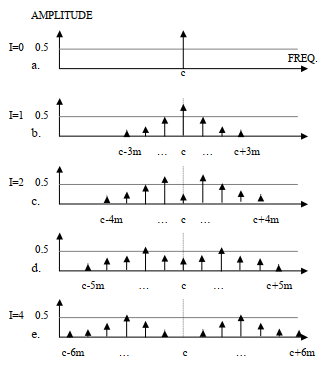
\includegraphics[width=0.4\textwidth]{ImagenesEjercicio3/Increasing-BW-I.png}
	\caption{Aumento de $I(t)$ y como afecta las frecuencias laterales.}
	\label{fig:Iaumenta}
\end{figure}

Las amplitudes de la portadora y las laterales son determinadas por las funciones de Bessel de primer y ``n-esimo'' orden $J_1 \left( I(t) \right)$ y $J_n \left( I(t) \right)$, expresando $x(t)$ de la forma:
\begin{equation}
	x(t) = A \ \sum_{0}^{n} J_k \left(I(t) \right) \ \left[ sen(\omega_c + k \omega_m)t - sen(\omega_c - k \omega_m)t \right]
\end{equation}

La principal ventaja de la síntesis mediante F.M. consiste justamente en el hecho de que se puede expresar con facilidad la relación entre la portadora y la moduladora, lo que produce las frecuencias laterales mencionadas previamente. Estas recaen en el lado negativo de frecuencias, reflejándose en el dominio positivo del espectro. 
\begin{figure}[H]
	\centering
	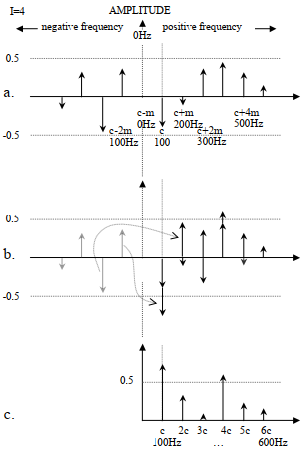
\includegraphics[width=0.4\textwidth]{ImagenesEjercicio3/Reflecting-f.png}
	\caption{Representación gráfica de la proyección de frecuencias negativas.}
	\label{fig:freflect}
\end{figure}

Por otro lado, se puede expresar la relación de la frecencia portadora y moduladora de la forma
\begin{equation}
	\frac{f_c}{f_m} = \frac{N_1}{N_2}
	\label{equ:cm}
\end{equation}
lo que permite obtener una expresión para la frecuencia central
\begin{equation}
	f_o = \frac{f_c}{N_1} = \frac{f_m}{N_2}
\end{equation}

\subsection{Instrumentos de viento}
Este método puede ser empleado para sintetizar instrumentos de viento, fijando los parámetros $A(t)$, $I(t)$, $f_c$ y $f_m$ de una forma adecuada. Existen modelos dados para ciertos instrumentos, los cuales pueden ser modificados para conseguir un sonido más fidedigno, siendo el principal parámetro la relación presentada en la Ecuación (\ref{equ:cm}).

\subsubsection{Clarinete}
Para al síntesis del clarinete se utilizó una relación $3 f_c  = 2 f_m$. Además, las funciones $A(t)$ e $I(t)$ para una señal de una duración de $1$ segundo son las presentadas a continuación.
\begin{figure}[H]
	\centering
	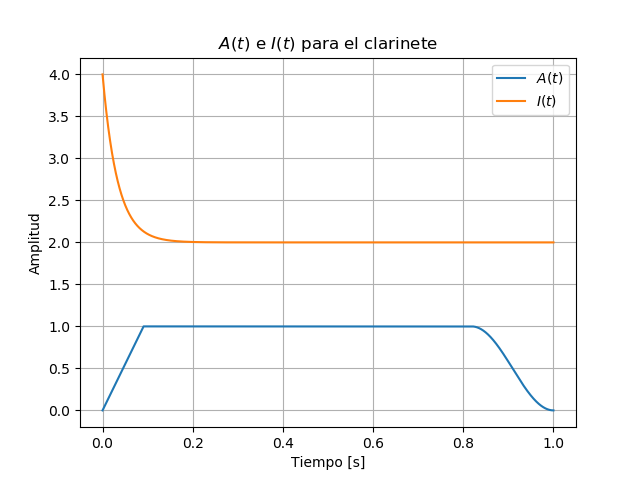
\includegraphics[width=0.7\textwidth]{ImagenesEjercicio3/A-I-Clarinet.png}
	\caption{$A(t)$ e $I(t)$ para un clarinete.}
	\label{fig:aiclar}
\end{figure}

Luego, se obtuvo un espectrograma para una nota a $440 \ Hz$ de dicho instrumento. Para dicho análisis se valió de una ventana de Hanning con 256 puntos para la $NFTT$ y una superposición de $128$.  
\begin{figure}[H]
	\centering
	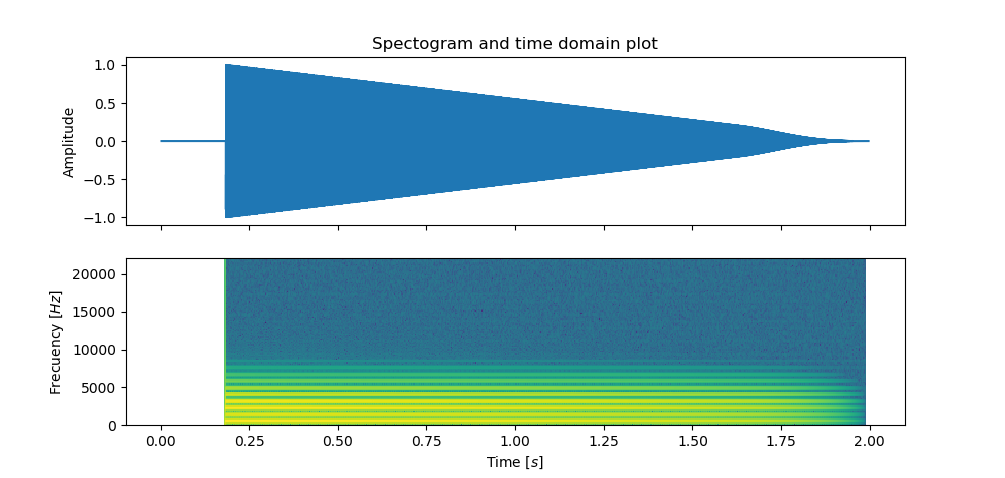
\includegraphics[width=0.9\textwidth]{ImagenesEjercicio3/Clarinet-440-Hanning-256-128.png}
	\caption{Espectrograma de una nota de clarinete a $440 \ Hz$.}
	\label{fig:specclar}
\end{figure}

\subsubsection{Trombón}
De manera similar al caso anterior, para al síntesis del trombón se utilizó una relación $f_c = f_m$. Además, las funciones $A(t)$ e $I(t)$ para una señal de una duración de $1$ segundo son las presentadas a continuación.
\begin{figure}[H]
	\centering
	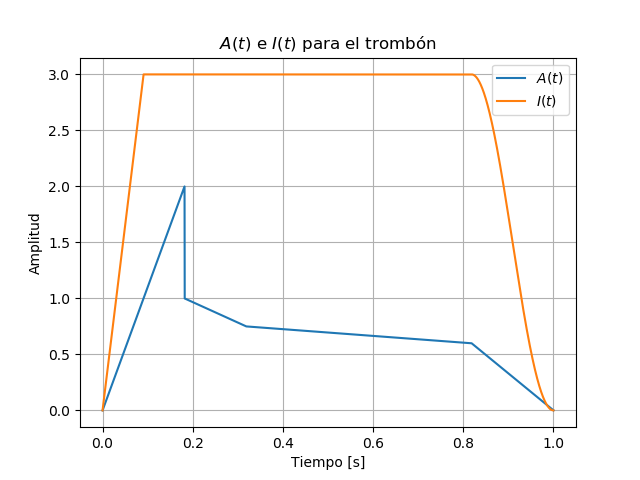
\includegraphics[width=0.7\textwidth]{ImagenesEjercicio3/A-I-Trombone.png}
	\caption{$A(t)$ e $I(t)$ para un trombón.}
	\label{fig:aitromb}
\end{figure}

Después, se obtuvo un espectrograma para una nota a $440 \ Hz$ de dicho instrumento. Para dicho análisis se valió de una ventana de Hanning con 256 puntos para la $NFTT$ y una superposición de $128$.  
\begin{figure}[H]
	\centering
	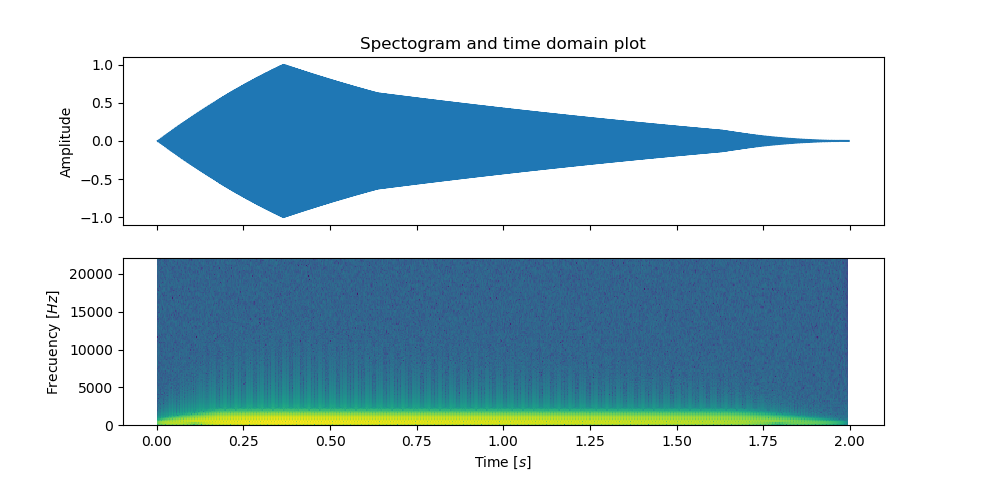
\includegraphics[width=0.9\textwidth]{ImagenesEjercicio3/Trombone-440-Hanning-256-128.png}
	\caption{Espectrograma de una nota de trombón a $440 \ Hz$.}
	\label{fig:spectromb}
\end{figure}

\subsubsection{Campana}
Analogamente, para la campana se empleó una relación $ f_c = 2 f_m$. Además, las funciones $A(t)$ e $I(t)$ para una señal de una duración de $1$ segundo son las presentadas a continuación.
\begin{figure}[H]
	\centering
	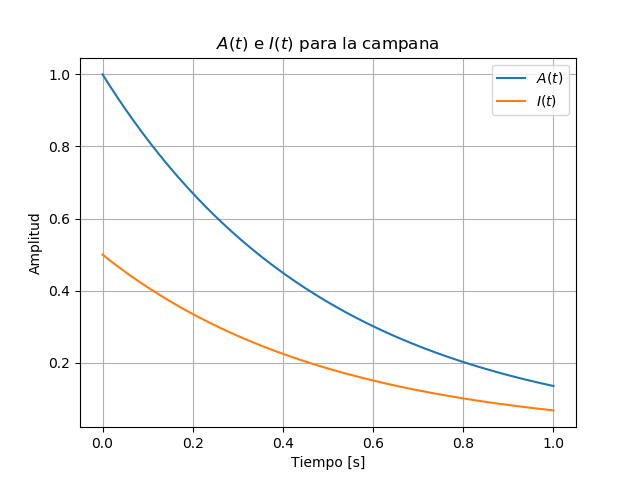
\includegraphics[width=0.7\textwidth]{ImagenesEjercicio3/A-I-Bell.png}
	\caption{$A(t)$ e $I(t)$ para una campana.}
	\label{fig:aibell}
\end{figure}

Luego, se desarrollo un espectrograma para una nota a $440 \ Hz$ de dicho instrumento. Para dicho análisis se valió de una ventana de Hanning con 256 puntos para la $NFTT$ y una superposición de $128$.  
\begin{figure}[H]
	\centering
	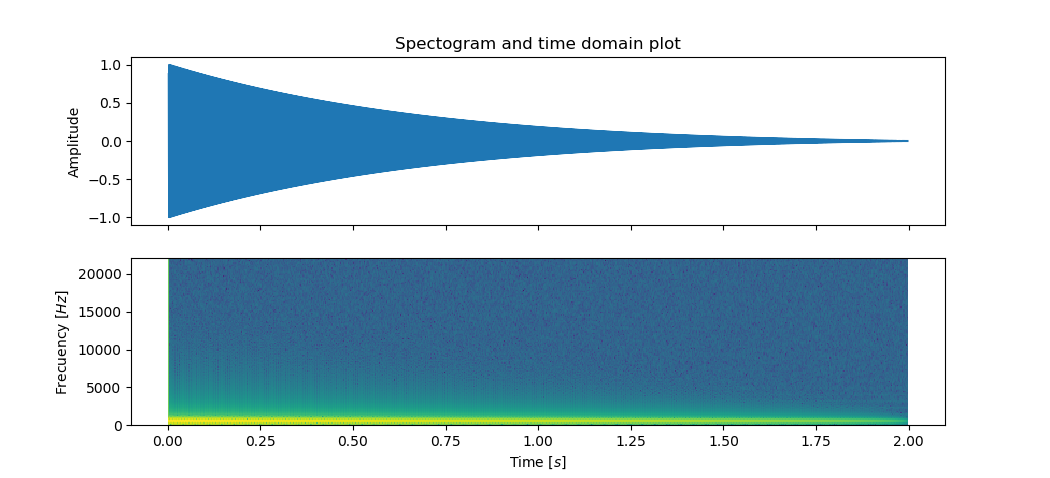
\includegraphics[width=0.9\textwidth]{ImagenesEjercicio3/Bell-440-Hanning-256-128.png}
	\caption{Espectrograma de una nota de campana a $440 \ Hz$.}
	\label{fig:specbell}
\end{figure}

\subsubsection{Trompeta}
Finalmente, para sintetizar una trompeta se utilizó la misma relación que para el trombón, $f_c = f_m$. Además, las funciones $A(t)$ e $I(t)$ para una señal de una duración de $1$ segundo son las presentadas a continuación.
\begin{figure}[H]
	\centering
	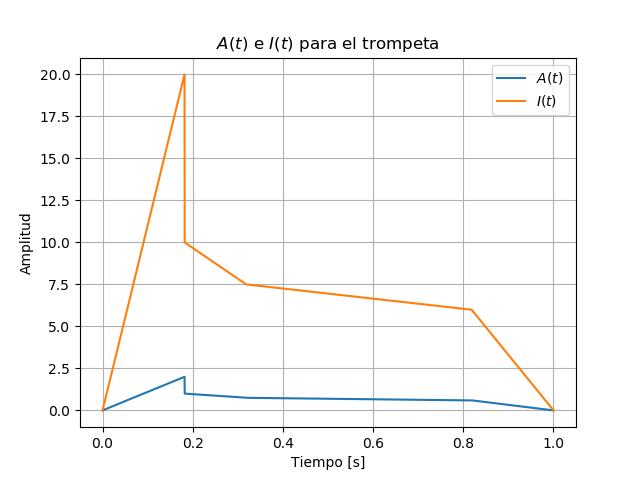
\includegraphics[width=0.7\textwidth]{ImagenesEjercicio3/A-I-Trumpet.png}
	\caption{$A(t)$ e $I(t)$ para una trompeta.}
	\label{fig:aitrumpet}
\end{figure}

Luego, se obtuvo un espectrograma para una nota a $440 \ Hz$ de dicho instrumento. Para dicho análisis se valió de una ventana de Hanning con 256 puntos para la $NFTT$ y una superposición de $128$.  
\begin{figure}[H]
	\centering
	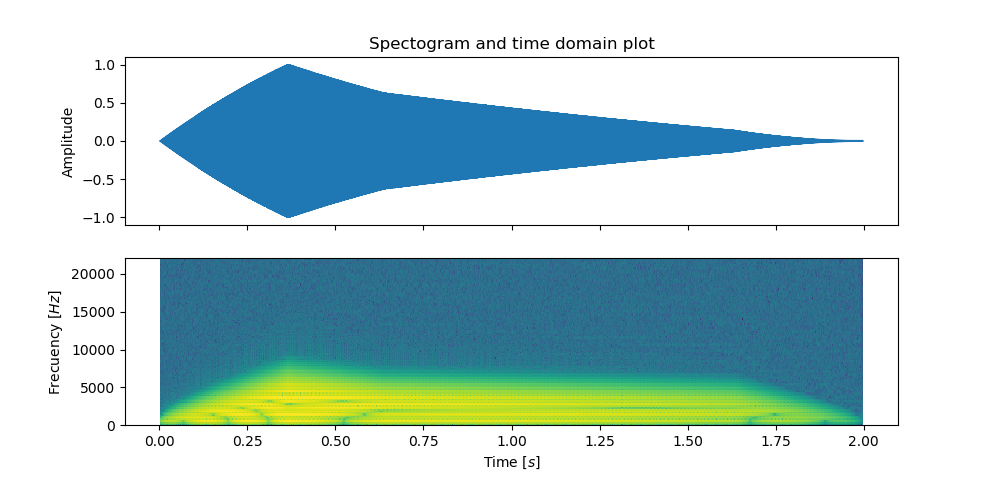
\includegraphics[width=0.9\textwidth]{ImagenesEjercicio3/Trumpet-440-Hanning-256-128.png}
	\caption{Espectrograma de una nota de trompeta a $440 \ Hz$.}
	\label{fig:spectrumpet}
\end{figure}
 
\subsection{Conclusiones}
No existe un acercamiento analítico para determinar el mejor conjunto de parámetros para la síntesis de un instrumento mediante el método de F.M., lo que dificulta la selección de estos \footnote{Andrew Horner y James W. Beauchamp, \href{https://www.researchgate.net/publication/226790075_Instrument_Modeling_and_Synthesis}{Instrument Modeling and Synthesis.} 2009.}. Es por ello que existen bases de como tratar cada instrumento, las cuales pueden ser libremente modificadas, dependiendo del gusto de cada persona, justificando la existencia variaciones de cada ``plantilla''. A pesar de ello, dichos cambios deben hacerse con cierto criterio, ya que se desea mantener un sonido similar al real, y provocar cambios sin tener conocimiento pueden generar sonidos muy distantes a los deseados.
\end{document}